\documentclass{article}

% New commands declaration

\usepackage[frenchb]{babel}
\usepackage[T1]{fontenc}

\usepackage{natbib,bibentry}
\usepackage{color}

\usepackage{yfonts}
\usepackage{graphicx}
\usepackage{epsfig,subfigure}
\usepackage{amsmath,amssymb,amsfonts}
\usepackage{calc, float}
\usepackage{import}
\usepackage{stmaryrd}


\DeclareGraphicsExtensions{.eps, .jpg, .png}

\parindent = 0mm

\bibliographystyle{plain}

\hoffset = -20mm
\voffset = -25mm
\textwidth = 160mm
\textheight = 240mm

\definecolor{lightgray}{gray}{0.2}

\newcommand{\expect}{{\rm I \mkern-2.5mu \nonscript\mkern-.5mu E}}
\newcommand{\equaldef}{\stackrel{d}{=}}
\newcommand{\argmax}{\operatornamewithlimits{argmax}}

\newcommand{\debutrep}[1]{\color{blue}\begin{center} \hrulefill \textbf{ #1 } \hrulefill \end{center} }
\newcommand{\finrep}{\vspace*{5mm}\hfill $\square$\color{black}\vspace*{5mm}}

\begin{document}

\baselineskip = 4mm
\title{Traitement des Signaux Aléatoires: \\
Prédiction linéaire d'un signal par modélisation Auto-Régressive \\
Application au débruitage}

\author{\textbf{4 ETI -- CPE Lyon }\\[3mm]
{Travaux Pratiques TSA}}
\date{}

\maketitle

\noindent\fbox{
\parbox{\linewidth-2\fboxrule-2\fboxsep}
{ 
\vspace*{2mm}
{\large\bf Noms, Prénoms: BURNOT Jean-Christophe, LANGUILLE Antoine }\\[3mm]
{\large\bf Groupe: D}\\[3mm]
{\large\bf Date: 13 décembre 2022}\\[2mm]}}
\vspace*{5mm}



{\Large\bf Objectif}~--~~\begin{minipage}[t]{135mm}
Débruitage d'un enregistrement sonore par prédiction linéaire basée sur un modèle auto-régressif.

\vspace*{4mm}
L'ensemble des fonctions Matlab nécessaires est à récupérer sur la  plateforme {\em CPe-campus} sous l'archive {\tt Fichiers\_TP\_AR.zip}.
\end{minipage}

\vspace*{4mm}
\renewcommand{\thesection}{\Roman{section}}

\section{Préparation : Modélisation auto-régressive d'un signal aléatoire}

Soient $(s_n,\,n=1,\ldots, N)$, les échantillons d'un signal aléatoire réel, stationnaire. On se propose de trouver \textbf{un modèle} tel que l'on puisse prédire linéairement la valeur de $s_n$  à partir des échantillons précédents de $s$
\begin{equation}
\hat{s}_n = \sum_{k=1}^{\infty} h[k]\,s_{n-k}.
\label{eq:AR(M)}\end{equation}
Il s'agit donc de déterminer les coefficients  $h[k]$, $k=1,2,\ldots$  minimisant l'erreur de prédiction:
\begin{equation}
\varepsilon_n = s_n - \hat{s}_n = s_n - \sum_{k=1}^{\infty} h[k] s_{n-k}
\label{eq:erreur}
\end{equation}
au sens de l'erreur quadratique  moyenne (i.e. puissance moyenne minimale) $P_{\varepsilon} = \mathbb{E}\{ \varepsilon^2_n\} = \sigma^2$

\subsection{}
Quel principe de construction  permet de garantir une erreur quadratique moyenne minimale? \\

\debutrep{réponse}
Le principe d'orthogonalité
\[
\begin{split}
    & \varepsilon_k \perp \hat{s}_k \\
    \Longleftrightarrow & \mathbb{E}(\varepsilon(n)\hat{s}(n)) = 0 \forall n \\
    \Longleftrightarrow & \mathbb{E}(\varepsilon(n)\sum_{m\ge1}h[m]s(n-m)) = 0 \ \ \ \forall n \\
    \Longleftrightarrow & \sum_{m\ge1}h[m]\mathbb{E}(\varepsilon(n)s(n-m)) = 0 \ \ \ \forall n \\
    \Longleftrightarrow & \forall n \ge 1; \ \mathbb{E}(\varepsilon(n)s(n-m))=0
\end{split}
\]
\finrep

\subsection{}
Par application de ce principe, montrer que l'erreur de prédiction $\varepsilon_n$ est  un bruit blanc.\\

\debutrep{réponse}
Le but est de montrer que $\varepsilon(n)$ est un bruit blanc.

C'est à dire qu'on cherche à arriver à:

$\mathbb{E}(\varepsilon(n)\varepsilon(m))=0 \text{ pour } n \ne m$

\[
\begin{split}
    \text{On a } & \mathbb{E} (\varepsilon(n)s(n-m))=0 \text{ avec } s(n) = \hat{s}(n)+\varepsilon(n) \\
    \Longleftrightarrow \  & \mathbb{E}(\varepsilon(n)(\varepsilon(n-m)+\sum_{k\geq1}^{}h[k]s(n-m-k))=0\\
    \Longleftrightarrow \ & \mathbb{E}(\varepsilon(n)(\varepsilon(n-m)+\varepsilon(n)\sum_{k\geq1}^{}h[k]s(n-m-k))=0\\
    \Longleftrightarrow \ & \mathbb{E}(\varepsilon(n)(\varepsilon(n-m)+\varepsilon(n)\sum_{k\geq1}^{}h[k]s(n-m-k))=0\\
    \Longleftrightarrow \ & \mathbb{E}(\varepsilon(n)(\varepsilon(n-m)+\sum_{k\geq1}^{}h[k]\mathbb{E}(\varepsilon(n)s(n-m-k)))=0\\
    & \text{Par le principe de l'orthogonalité } \mathbb{E}(\varepsilon(n)s(n-m-k))=0\\
    \\
    \text{On obtient alors: } & \mathbb{E}(\varepsilon(n)\varepsilon(n-m))=0\\
    \text{Par définition: } & \mathbb{E}(\varepsilon(k)^2)=P_\varepsilon = \sigma^2 \\
    & \mathbb{E}(\varepsilon(k)\varepsilon(l))=\sigma^2\delta_{n,l} \\
    & \mathbb{E}(\varepsilon(n)\varepsilon(n-m))=\sigma^2\delta[m]
\end{split}
\]
Nous sommes donc bien en présence d'un bruit blanc.
\finrep

\subsection{}
\label{eq.3} 
En pratique, il faut limiter  l'ordre du modèle à $M<\infty$. Dans ces conditions et toujours par application de ce même principe de construction, établir le système d'équations linéaires, dont les coefficients $\{h[k],~k=1,\ldots M\}$ sont les solutions.\\

\debutrep{réponse}
En limitant $k \leq M < +\infty$:

\[
\begin{split}
    & \mathbb{E}\left(\varepsilon(n) s(n-m)\right) = 0 \ \ \ \forall m \in \llbracket 1, M\rrbracket \\
    \Longleftrightarrow \ & \mathbb{E}( ( s(n)-\hat{s}\{n\})s(n-m) = 0 \\
    \Longleftrightarrow \ & \mathbb{E}(s(n) - s(n-m)) - \mathbb{E}(\hat{s}(n)s(n-m)) \\
    \Longleftrightarrow \gamma_S(m) &= \mathbb{E}\left(\sum_{K=-1}^M h[k]\mathbb{E}\left(s(n-k)s(n-m)\right)\right)\\
    &= \sum_{k=1}^M h[k] \gamma_S(k-m)\\
\end{split}
\]
On a alors
\[
\leftb
\begin{cases}
0 &= \gamma_s(1) - \left( h[1]\gamma_S(0) + h[2]\gamma_S(1) + \hdots + h[M]\gamma_S(M-1) \right)\\
0 &= \gamma_s(2) - \left( h[1]\gamma_S(1) + h[2]\gamma_S(0) + \hdots + h[M]\gamma_S(M-2) \right)\\
&\vdots\\
0 &= \gamma_s(M) - \left(h[1]\gamma_S(M-1) + h[2]\gamma_S(M-2) + \hdots + h[M]\gamma_S(0) \right)\\
\end{cases}
\]
On met alors ce système sous forme matricielle:
\[
-
\begin{pmatrix}
\gamma_S(1) & \gamma_S(0) & \hdots & \gamma_S(M-1) \\
\gamma_S(2) & \gamma_S(1) & \hdots & \gamma_S(M-2) \\
\vdots & \vdots & \ddots & \vdots \\
\gamma_S(M) & \gamma_S(M-1) & \hdots & \gamma_S(0) \\
\end{pmatrix}
\begin{pmatrix}
-1 \\ h[1] \\ h[2] \\ \vdots \\ h[M]
\end{pmatrix}
=
\begin{pmatrix}
0 \\ \vdots \\ 0
\end{pmatrix}
\]
\finrep


\subsection{}
Calculer la puissance de l'erreur de prédiction $P_{\varepsilon}$ en fonction de l'autocorrélation $\gamma_s(k)$ du signal et des coefficients $\{h[k],~k=1,\ldots M\}$.\\


\debutrep{réponse}
\[
\begin{split}
    \text{On a } \bar{P_\epsilon} &= \mathbb{E}(\varepsilon(n)^2)=\mathbb{E}((s(n)-\hat{s}(n))(s(n)-\hat{s}(n)))\\
    &= \mathbb{E}(s(n)(s(n)-\hat{s}(n)))-\mathbb{E}(\hat{s}(n)(s(n)-\hat{s}(n)))\\
    \text{Par principe d'orthogonalité:}\\
    &= \mathbb{E}(s(n)^2)-\mathbb{E}(s(n)\hat{s}(n))\\
    &= \mathbb{E}(s(n)^2)-\sum_{k=1}^M h[k]\mathbb{E}(s(n)s(n-k))\\
    &= \gamma_s(0)-(h[1]\gamma_s (1)+h[2]\gamma_s (2)+\hdots+h[m]\gamma_s (M)) \\
    \text{Or } P_\varepsilon = \sigma^2 \\
    \text{Donc} \sigma^2 &= \gamma_s(0)-(h[1]\gamma_s (1)+h[2]\gamma_s (2)+\hdots+h[m]\gamma_s (M))
\end{split}
\]
\finrep

\subsection{}
\label{eq.5}
Insérer cette relation dans le système 	d'équations linéaires  obtenu à la question \ref{eq.3}.\\

\debutrep{réponse}
En insérant l'expression précédente dans le système d'équations précédent, on obtient le système de Yule-Walker:
\[
\begin{pmatrix}
\gamma_S(0) & \gamma_S(1) & \hdots & \gamma_S(M) \\
\gamma_S(1) & \gamma_S(0) & \hdots & \gamma_S(M-1) \\
\gamma_S(2) & \gamma_S(1) & \hdots & \gamma_S(M-2) \\
\vdots & \vdots & \ddots & \vdots \\
\gamma_S(M) & \gamma_S(M-1) & \hdots & \gamma_S(0) \\
\end{pmatrix}
\begin{pmatrix}
-1 \\ h[1] \\ h[2] \\ \vdots \\ h[M]
\end{pmatrix}
=
\begin{pmatrix}
-\sigma^2 \\ 0 \\ \vdots \\ 0
\end{pmatrix}
\]
\[
\Longleftrightarroww
\begin{pmatrix}
\gamma_S(0) & \gamma_S(1) & \hdots & \gamma_S(M) \\
\gamma_S(1) & \gamma_S(0) & \hdots & \gamma_S(M-1) \\
\vdots & \vdots & \ddots & \vdots \\
\gamma_S(M) & \gamma_S(M-1) & \hdots & \gamma_S(0) \\
\end{pmatrix}
\begin{pmatrix}
\Phi[0] \\ \Phi[1] \\ \vdots \\ \Phi[M]
\end{pmatrix}
=
\begin{pmatrix}
1 \\ 0 \\ \vdots \\ 0
\end{pmatrix}
\text{Avec }
\Phi[k]
\leftb
\begin{cases}
    \frac{1}{\sigma^2}    & \text{Si } k = 0 \\
    -\frac{h[k]}{\sigma^2} & \text{sinon}
\end{cases}
\]
\finrep


\clearpage
\section{Manipulation}

\subsection{Signal et contexte}
Charger le signal audio {\tt ProtestMonoBruit.wav} avec la commande:\\[1mm]
{\tt
[s,Fs]= audioread('ProtestMonoBruit.wav') ;\\[1mm]
}
où $s$ et $Fs$ correspondent respectivement au signal échantillonné et à la fréquence d'échantillonnage.

En indiquant le code correspondant, afficher le signal (axe temporel gradué en secondes). Les pics aléatoires superposés au signal sont une affection classique des sons numérisés à partir de disques vinyles, qui se manifestent par un  \textit{bruit de craquement} lorsqu'on écoute le fichier audio:\\[1mm]
{\tt
sound(s,Fs) ;\\[2mm]
}

\debutrep{code}
\begin{verbatim}
%% TP4: Filtrage de Wiener
clear variables;
close all;
clc;

[s,Fs]= audioread("ProtestMonoBruit.wav");
x = 0 : 1/Fs : 1/Fs * (length(s)-1);

% Affichage du signal
figure();
plot(x,s);
title("Signal brut");
xlabel("temps (s)");
ylabel("Amplitude");

sound(s, Fs);
\end{verbatim}
\finrep

\debutrep{figures}
\begin{figure}[H]
    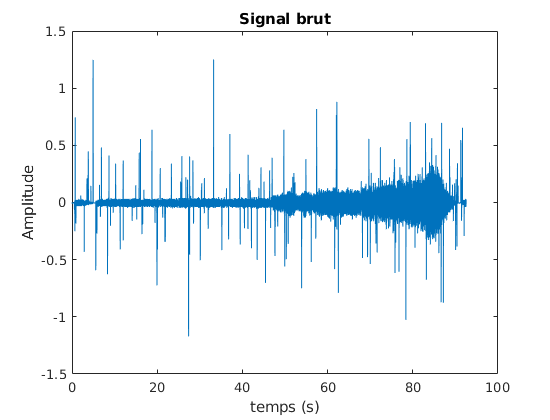
\includegraphics[width=\columnwidth]{signal.png}
    \caption{Signal d'origine bruité}
\end{figure}
\finrep

On se propose de restaurer le signal initial en {\em débruitant} l'enregistrement.\\
Quelle(s) solution(s) simple(s) pourrait on envisager pour supprimer (ou atténuer) l'effet de ces pics? En quoi ne seraient elles pas satisfaisantes?

\debutrep{réponse}
Nous pouvons envisager plusieurs solutions pour supprimer ces pics:
\begin{itemize}
    \item Un filtrage passe-bas permettant de supprimer les hautes fréquences, mais ce dernier atténue aussi les hautes fréquences du signal. Le son produit en sortie est alors "étouffé".
    
    \item Un seuillage en amplitude: si le signal dépasse une certaine amplitude on remplace les échantillons par une valeur moyenne ou médianne calculée localement avec le signal. Le prin,cipal problème vient lorsque le signal a une forte amplitude, le seuil devrait alors être "adaptatif" au signal.
    
\end{itemize}
\finrep

\vspace*{3mm}
La solution retenue ici, consiste à modéliser l'enregistrement audio (qui n'est pas un bruit blanc!) par un \textbf{processus auto-régressif d'ordre M }($AR(M)$). Ce modèle est ensuite utilisé pour prédire l'échantillon  $s_n$ du signal à partir des $M$ échantillons précédents $\{s_{n-m},\,1 \leq m \leq M)\}$ . Puisque l'apparition des pics de craquement est \textbf{aléatoire} et supposée \textbf{indépendante} du signal, le modèle $AR(M)$ n'aura pas le pouvoir de  les prédire.


\subsection{Estimation de la fonction d'autocorrélation.}

Pour limiter les temps de calcul, on limitera l'analyse du signal à l'intervalle $t\in[60,70]$ secondes. \\
Sur ce segment, estimer la fonction d'autocorrélation $\gamma_s[k] = \gamma_s(kTs)$, 
% (avec $\gamma_s(0)=1$), 
pour $-K\leq k \leq K$. Pour cela, on utilisera l'instruction suivante:  {\tt [R,lags] = xcorr(x,K,'biased')}, où $R$ est le vecteur des corrélations et {\tt lags}, le vecteur des retards $-K\leq k \leq K$. Afficher le code correspondant et le résultat pour $K=200$ (on n'hésitera pas à faire un zoom autour de la zone d'intérêt\ldots) 

\debutrep{code}
\begin{verbatim}
%% Calcul de l'autocorrelation du signal

% on se limite aux intervalles [60s, 70s]
t = x( (60 <= x) & (x <= 70) );
S = s( (60 <= x) & (x <= 70) );

K = 200;

[R, lags] = xcorr(S, K, 'biased');

figure();

stem(lags, R);
title(sprintf("Autocorrelation K=%d", K));
xlabel("Retard (k)");
ylabel("Amplitude");
grid on;
\end{verbatim}
\finrep

\debutrep{figures}
\begin{figure}[H]
    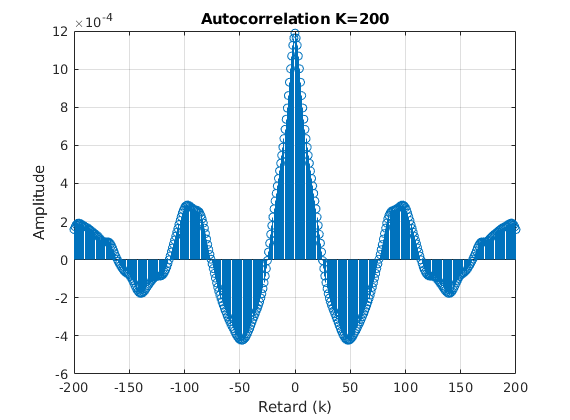
\includegraphics[width=0.9\columnwidth]{xcorr.png}
    \caption{Autocorrélation du signal $\gamma_s(\tau)$}
\end{figure}
\begin{figure}[H]
    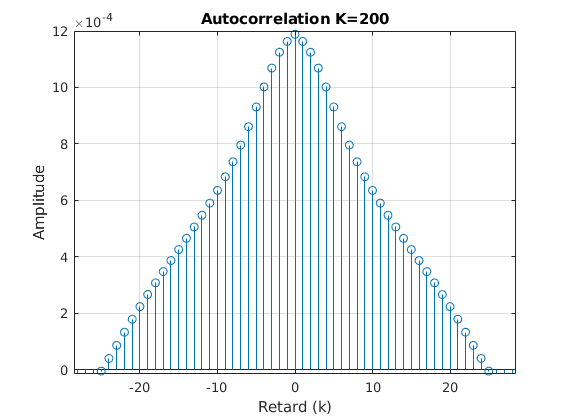
\includegraphics[width=0.9\columnwidth]{xcorr-zoom.png}
    \caption{Zoom sur la partie centrale de $\gamma_s(\tau)$}
\end{figure}
\finrep

A partir de cette fonction, justifier le choix $M \approx 20$ pour l'ordre du modèle $AR(M)$.

\debutrep{réponse}
Avec le tracé de notre autocorrélation on mesure un rayon de corrélation de $\tau_c \approx 25$ (premier passage par zéro de $\gamma_S(\tau)$. De plus notre signal est de plus pseudo-stationnaire (stationnaire sur un intervalle restreint)

On se limitera alors sur l'intervalle $\tau \in \llbracket -20,20 \rrbracket$ pour $\gamma_S(\tau)$ pour économiser les calculs ainsi que conserver l'hypothèse de pseudo-stationnarité.
\finrep

\subsection{Identification du modèle $AR(M)$}

En fixant alors l'ordre du modèle auto-régressif à $M=20$, programmer et résoudre l'équation matricielle (complète) obtenue à la question  \ref{eq.5} de la préparation. Utiliser pour cela, la fonction {\tt toeplitz.m} de Matlab. \\[1mm]
\textbf{Note:} $\gamma_s$ est la fonction d'autocorrélation  \textbf{empirique} estimée à partir des échantillons de $s$. La matrice de Toeplitz de la question \ref{eq.5} de la préparation peut donc ne pas être inversible. On utilisera alors la commande {\tt pinv.m} de Matlab pour calculer la matrice pseudo-inverse (de Moore-Penrose) qui elle, existe toujours.\\[1mm]
Reproduisez ci-dessous, le code développé pour le calcul des coefficients.

\debutrep{code}
\begin{verbatim}
% Taille de la matrice
M = 20;

% Création de la matrice d'intercorrélation
gamma = R( (0<= lags) & (lags <= M) );
G = toeplitz(gamma);

y = zeros(M+1, 1);
y(1) = 1;

% On résoud le systême G * h = y
% en "inversant" la matrice G
Gi = pinv(G);

res = Gi * y;
sigma = sqrt(1/res(1));
h = -sigma^2 * res(2 : end);

figure();
stem(h);
title("Coefficients h[k]");
xlabel("Indice (k)");
ylabel("Amplitude");
\end{verbatim}
\finrep

Afficher les coefficients  du modèle $AR(M)$ $\{h[k],~k=1,\ldots M\}$ ainsi obtenus.

\debutrep{figures}
\begin{figure}[H]
    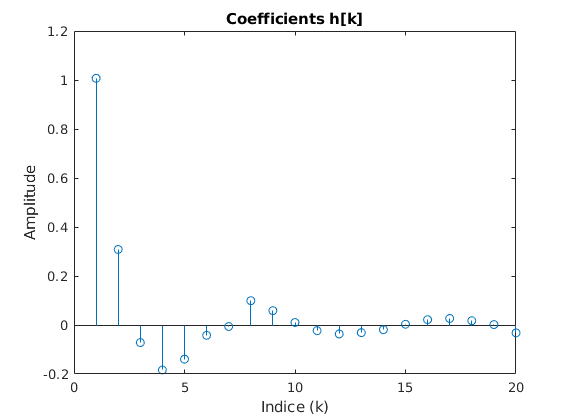
\includegraphics[width=\columnwidth]{coefs-h.png}
    \caption{Réponse impulsionnelle du filtre $h[k]$}
\end{figure}
\finrep

\subsection{Prédiction linéaire}
\label{sec:predlin}

En utilisant les coefficients $(h[k],~k=1,\ldots,M)$ du modèle $AR(20)$ ainsi identifié, calculer la prédiction à un pas de temps $\hat{s}_n$ de $s_n$ à partir des échantillons précédents $(s_{n-k},~k=1,\ldots,M)$, pour $n \geq M+1$.\\[1mm]
Reproduisez ci-dessous, le code développé pour effectuer la prédiction et le calcul de l'erreur de prédiction.

\debutrep{code}
\begin{verbatim}
%% Prédiction du signal

Sp = [zeros(M,1); conv(S, [0; h], "valid")];

figure();
subplot(2,1,1);

stem(t, S);
hold on;
stem(t, Sp);
title("Comparaison des signaux");
legend("Brut", "Prédit");
xlabel("Temps (s)");

subplot(2,1,2);
stem(t, abs(S-Sp));
title("Erreur d'estimation");
xlabel("Temps (s)");
\end{verbatim}
\finrep

Afficher (en {\tt subplot(211)}) la prédiction du signal ainsi obtenue superposée au  signal original et faites un zoom sur un craquement de votre choix.

Sur la même figure (en {\tt subplot(212)}) afficher la valeur absolue de l'erreur de prédiction $\varepsilon_n = \hat{s}_n - s_n$.

\debutrep{figures}
\begin{figure}[H]
    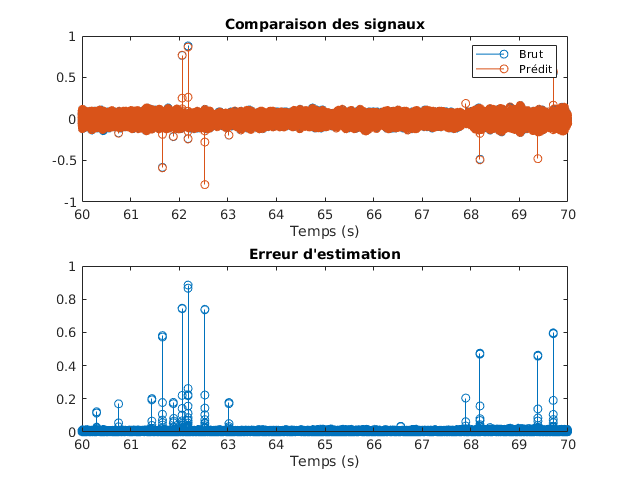
\includegraphics[width=0.857\columnwidth]{prediction-erreur.png}
    \caption{Comparaison et erreur des signaux réels (bleu) et prédit par filtrage (bleu)}
\end{figure}
\begin{figure}[H]
    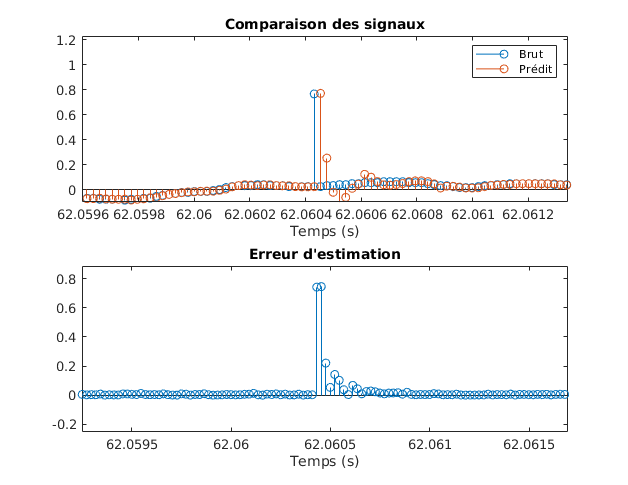
\includegraphics[width=0.9\columnwidth]{prediction-erreur-zomm.png}
    \caption{Zoom sur un pic du signal}
\end{figure}
\finrep

\subsection{Restauration par seuillage}

Choisissez un seuil $\Sigma$ pour identifier à partir de l'erreur de prédiction, les indices $k_i$ des dates de craquement.  Pour chacun de ces indices,  remplacer la valeur $s_{k_i}$ (i.e. craquement) par la valeur médiane (fonction {\tt median.m} sous Matlab) des échantillons de $s$ situés autour de $k_i$, $\{s_{k_i+l},~l=-10, -9,\ldots, 0 , \ldots 10\}$.

\debutrep{code}
\begin{verbatim}
% Correction
seuil = 5*sigma;

%cracks = abs(S - Sp) > seuil;
%Sc = Sp .* cracks + S .* (1 - cracks);

Sc = S;
for i=M:length(S)
    if abs(S(i) - Sp(i)) > seuil
        Sc(i) = median(S( i-10 : i+10 )); 
    end
end


figure();
stem(t, S);
hold on;
stem(t, Sc);
title("Signal corrigé");
legend("Brut","Corrigé");
xlabel("Temps (s)");
%xlim([62.06, 62.061]);

sound(Sc, Fs);
\end{verbatim}
\finrep

Afficher le signal ainsi restauré  superposé au signal original bruité (faire un zoom sur la même plage de signal qu'à la question \ref{sec:predlin}).\\

\debutrep{figures}
\begin{figure}[H]
    \includegraphics[width=\columnwidth]{causal-corrige.png}
    \caption{Signal corrigé avec erreur basée sur filtrage causal}
\end{figure}
\begin{figure}[H]
    \includegraphics[width=\columnwidth]{causal-corrige-zoom.png}
    \caption{Zoom sur un pic du signal non filtré}
\end{figure}
\finrep

Ecouter le signal restauré. Commentez.

\debutrep{réponse}
Les pics (craquements) sont bien moins présent que sur le signal d'origine. Néanmoins le son reste abimé, en effet, même si les pics ne sont plus présents, il reste un des zones perturbés qui se trouvent aux environs des pics. Ces zones perturbés sont celles qui induisent des imperfections dans notre son.
\finrep


\subsection{Restauration par prédiction {\em causale / anticausale}}

La prédiction causale (estimation de l'échantillon $s[n]$ à partir des échantillons antérieurs) de la question \ref{sec:predlin} produit une erreur de prédiction où chaque craquement est repéré par un pic principal, suivi d'un train de pics secondaires (rebonds dus au temps de réponse du filtre $h[k]$). Le débruitage par seuillage de cette erreur de prédiction peut alors conduire à la détection de faux craquements\ldots
Pour éviter cela, on peut procéder à une prédiction causale, combinée à une prédiction anticausale où chaque échantillon 
$s[n]$ est prédit à partir des $M$ échantillons suivants $(s[n+k],\,k=1,\ldots,M)$ et ce, en utilisant le même filtre $h[k]$ puisque la fonction d'autocorrélation est paire. Les erreurs de prédiction $\varepsilon_{\rm causale}$ et $\varepsilon_{\rm anticausale}$ n'ont alors en commun que les pics principaux localisés aux instants des craquements. Il suffit ensuite de remplacer l'échantillon $s[n_{\rm crack}]$ par la moyenne des deux prédictions $\widehat{s}_{\rm causal}[n_{\rm crack}]$ et $\widehat{s}_{\rm anticausal}[n_{\rm crack}]$. \\

Programmez cette solution en expliquant bien chaque étape de la procédure. 

\debutrep{code}
\begin{verbatim}
% Correction double
seuil = 5*sigma;

Sc = S;
for i=1:length(S)
    if abs(S(i) - Sp(i)) > seuil && abs(S(i) - Spa(i)) > seuil
        Sc(i) = (Sp(i) + Spa(i)) /2;
    end
end

figure();
stem(t, S);
hold on;
stem(t, Sc);
title("Signal corrigé");
legend("Brut","Corrigé");
xlabel("Temps (s)");
%xlim([62.06, 62.061]);
\end{verbatim}
\finrep

Affichez le résultat de la restauration ainsi obtenue.

\debutrep{figures}
\begin{figure}[H]
    \includegraphics[width=0.85\columnwidth]{dual-corrige.png}
    \caption{Signal corrigé avec correction basée sur filtrage causal et anticausal}
\end{figure}
\begin{figure}[H]
    \includegraphics[width=0.85\columnwidth]{dual-corrige-zoom.png}
    \caption{Zoom sur un pic du signal non filtré}
\end{figure}
\finrep

Ecoutez le signal restauré. Concluez.

\debutrep{réponse}
Le son semble dépourvu d'imperfections. La restauration basée sur le filtrage causal et anticausal n'a affecté que les échantillons où se trouvaient les craquements en préservant les autres échantillons. La restauration est donc quasi parfaite.

On ne peut cependant pas récupérer l'information perdue mais on peut suffisament l'approcher 
\finrep

\end{document}
